%Correct the file name.
%X: book number
%Y: part number
%ZZZ: page number in three digits. So page 3 would be 003.

\documentclass[11pt]{amsbook}

\usepackage{../HBSuerDemir}	% ------------------------


\begin{document}

% ++++++++++++++++++++++++++++++++++++++
\hPage{ceyhun/051}
$\overline{A}= \hAbs{a_{ij}}_{a.a} \underline{ayrıt \ matrisi}, i \neq j $ için, eğer i ninci ayrıt j ninci ayrıta bitişik ise (bitişik değil ise )  $ a_{ij}= 1$ ( 0 ) $ i=j$ için $a_{ii}=2$ olarak tanımlanır.
\begin{defn}
    ${\Large Ç}(d,a)$ çizgisinin a dizek ve a dikeçten oluşan, \\
    $\overline{A}=\hPairingBraket{a_{aj-}}_{a.a}$
    \underline{indirgenmiş ayrıt matrisi} $ A = \overline{A} - 2 {\Large I_{a}}$ olarak tanımlanır.
\end{defn}
İndirgenmiş ayrıt matrisinden köşegen öğelerin sıfır olduğu gözden kaçmamalıdır. Tanım 2.1.7 de $ {\Large I_{a}} , \  a\times a  $ boyutundaki birim matrisi göstermektedir. Yukarda verdiğimiz tanımlardan , bu matrislerin de  bakışımlı olduğu, 
\begin{align*}
\overline{A} &= \overline{A}' \\
A&=A'
\end{align*}
ve
\begin{align*}
\overline{A} &= P'P
\end{align*}
eşitliği görülebilir (gösteriniz). Şekil 2.1.1a daki çizgiye ilişkin düğüm ve ayrıt matrisleri



\end{document}


%==== environments ====

%\begin{figure}[htb]
%	\centering
%	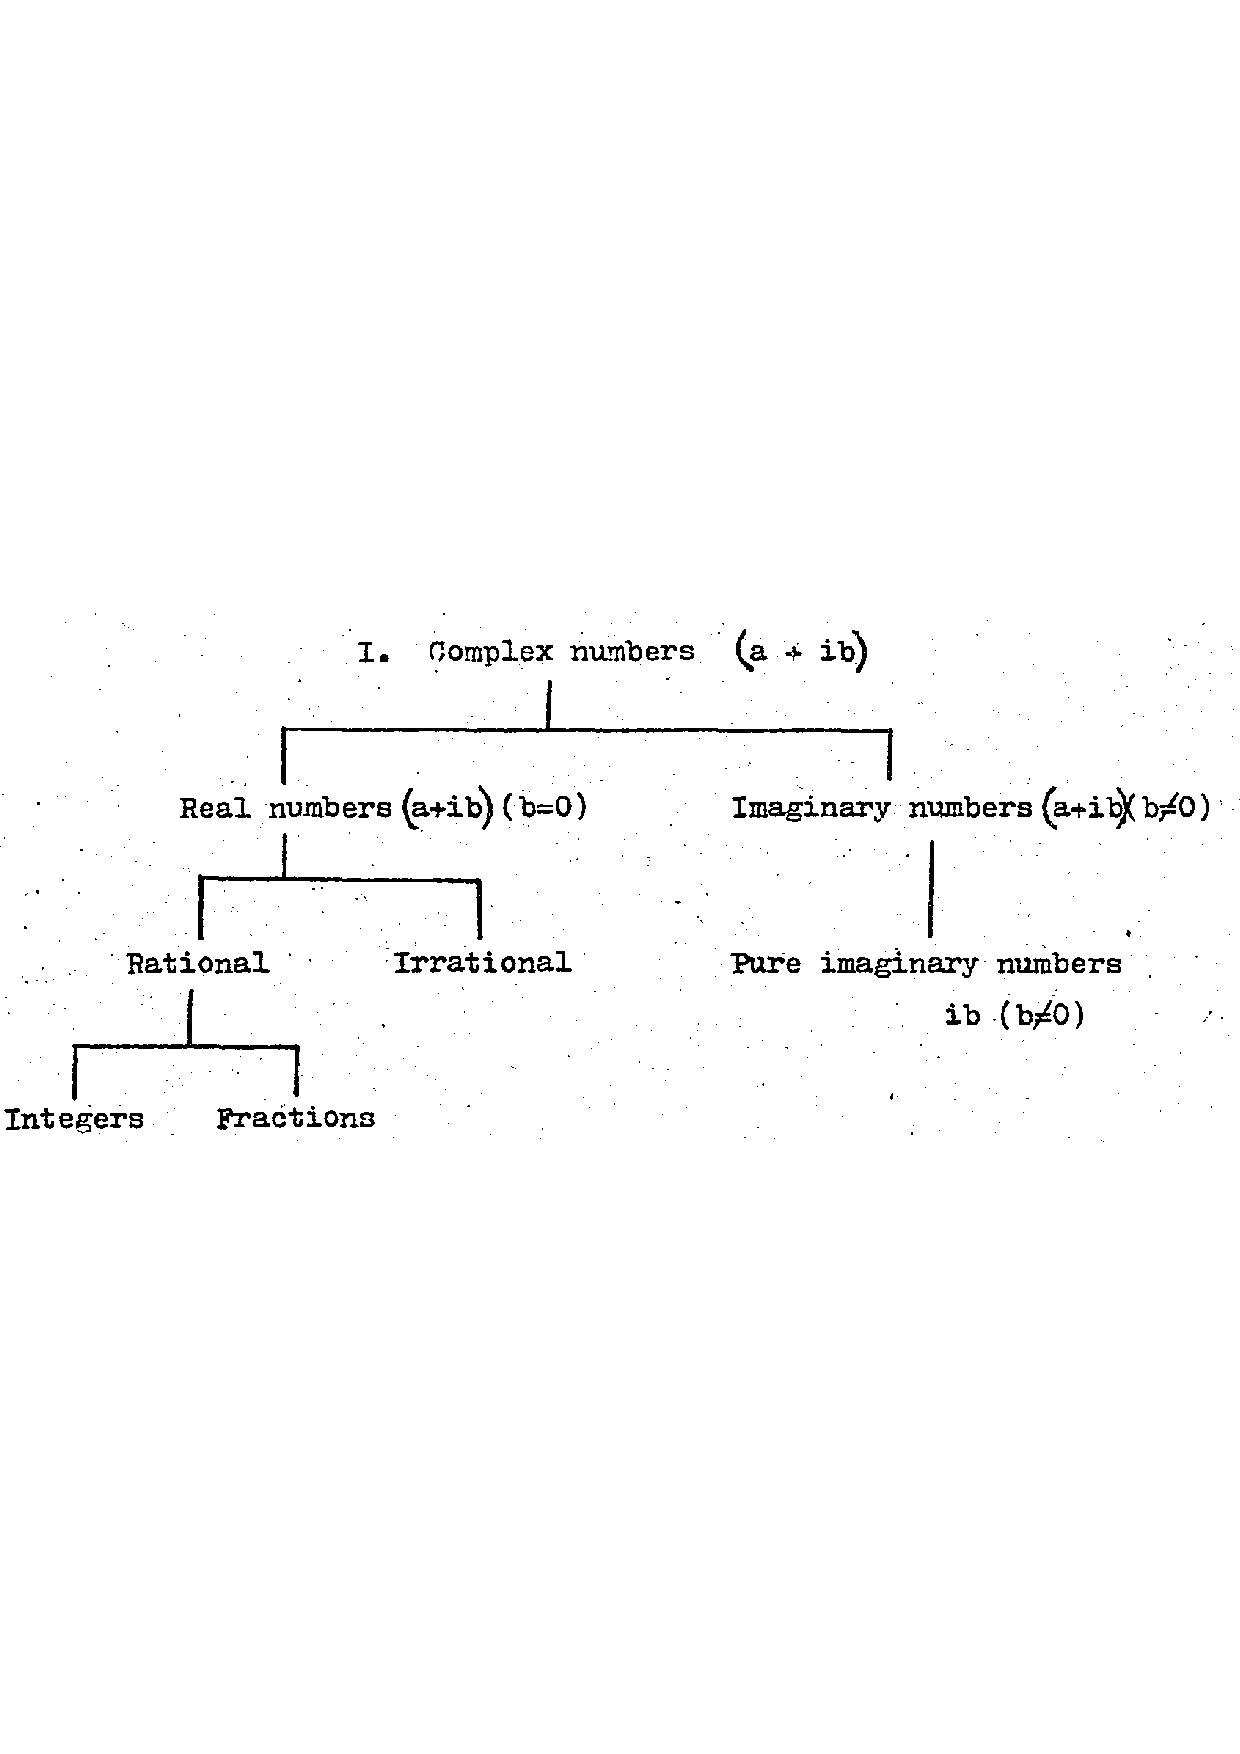
\includegraphics[width=0.9\textwidth]{images/SD-1-1p15A}
%	\caption{Classification of complex numbers}
%	\label{fig:classificationOfComplexNumbersA}
%\end{figure}

%\begin{center}
%\begin{tabular}{cc}
%\end{tabular}
%\end{center}

%\begin{exmp}
%\begin{hSolution}
%\end{hSolution}
%\end{exmp}

%\begin{hEnumerateAlpha}
%\end{hEnumerateAlpha}

%\begin{hEnumerateRoman}
%\end{hEnumerateRoman}

%$
%\begin{bmatrix}
%\end{bmatrix}
%$

%\frac{aaaa}{bbb}
%\frac{a_{n}}{b_{n}}
%\left( aaaa \right)
%\Longrightarrow

%\begin{multicols}{2}
%	bb
%\columnbreak
%	aa
%\end{multicols}
